% !TEX root = main.tex

\chapter{Theoretical framework}
Quantum computing is based on a general framework that does not depend on the physical platform. Here, important concepts such as qubit, and quantum operations are described from a theoretical point of view, before showing how we can realize them with trapped ions. The same goes with quantum networking, the concept and the realization can be treated separately and they will be described in this chapter. Furthermore, in this chapter we will take a look into Gaussian beams and their properties. Since that is the shape emitted by laser, it is important to understand their characteristic and how to manipulate them. Lastly, Acousto-optical interactions are introduced and studied to give an idea of how AODs work and how they can be used to steer a laser beam.
\section{Quantum logic with trapped ions}
\subsection{Quantum computer and quantum gates}
The concepts of quantum computing are borrowed and extended from classical computational theory. In the classical case, information is mostly represented in terms of binary digits, the so called bit, essentially mapping information to a base-2 number. Information processing is done with gates acting of those numbers. The idea of quantum computer is still to encode information in a binary form, but due to the nature of quantum mechanics, a quantum bit (in short qubit) gains new features that can be exploited to perform different kind of operations.\\
A qubit is formally a normalized wave function that can be written as superposition of two orthogonal states indicated usually with $\ket{0}$ and $\ket{1}$:
\begin{equation}
\label{qubit}
\ket{\psi} = \alpha \ket{0} + \beta\ket{1},
\end{equation}
where $\alpha,\beta$ are probability amplitudes, two complex numbers that satisfy the relationship $|\alpha|^2+|\beta|^2 = 1$.
At first glance, the advantage of qubits seems obvious, while one classical bit can store only one bit of information, a qubit can be in any linear combination, i.e. $\alpha$ and $\beta$ can be chosen freely and any information can be represented. Although, the reality is different, due to rules of quantum mechanics, $\alpha$ and $\beta$ cannot be directly accessed, which means that we can get only a limited amount of information out of a qubit. The outcome of measuring a qubit will give the value 0 with a probability of $|\alpha|^2$ and 1 with a probability of $|\beta^2|$.\\
Qubits also have a geometrical representation that can be useful, equation \eqref{qubit} depends on 4 real numbers, however since $\psi$ is normalized, we can rewrite the expression as
\begin{equation}
\ket{\psi} = e^{i\gamma}\left(\cos\frac{\theta}{2}\ket{0} + e^{i\varphi}\sin\frac{\theta}{2}\ket{1}\right).
\end{equation}
the global phase factor $e^{i\gamma}$ can be left out, as it does not influence the measurement outcome. This leaves us with only two real number: $\theta$ and $\varphi$. A qubit is therefore representable with only these two numbers that we can chose to represent geometrically with normalized spherical coordinates. The so called Bloch sphere is depicted in figure \ref{blochsphere}, every point on its surface represents a different state of the qubit. Here qubit manipulation can be visualized as trajectories on the surface. The drawback of this representation is that it is limited to only one qubit, so it loses usefulness when dealing with multiple qubits.
\begin{figure}[H]
\centering
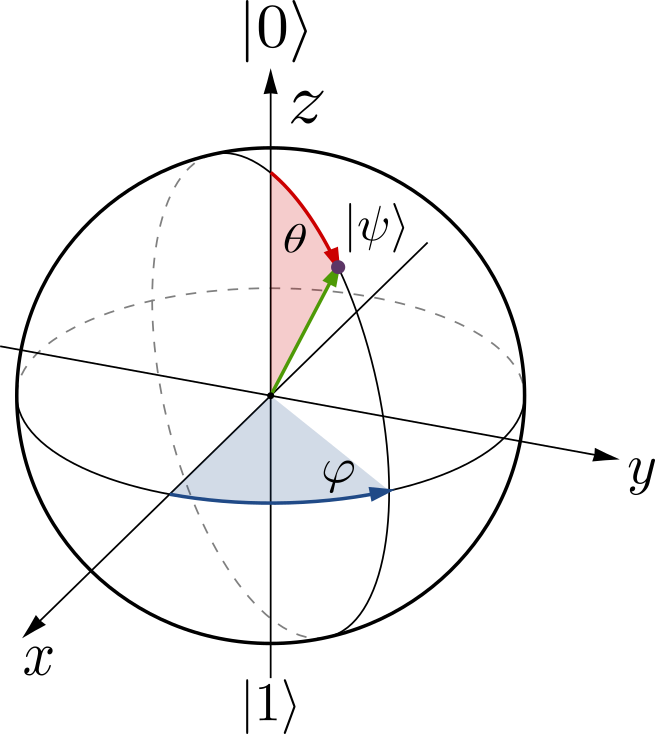
\includegraphics[width = .4\textwidth]{bloch_sphere}
\caption{The Bloch sphere. The states $\ket{0}$ and $\ket{1}$ are at the poles of the sphere, every other point of the surface represents a superpositions of these states. A quantum gate can be seen as trajectory on the surface mapping one state to another.}
\label{blochsphere}
\end{figure}

An alternative way of dealing with qubits is via matrices. We can assign to the states $\ket{0}$ and $\ket{1}$ the following:
\begin{equation}
\ket{0} = \begin{pmatrix}
 1 \\
 0
\end{pmatrix} \quad
\ket{1} = \begin{pmatrix}
 0 \\
 1
\end{pmatrix} \implies \ket{\psi} = \begin{pmatrix}
 \alpha \\
 \beta
\end{pmatrix}.
\end{equation}
In this representation, rotations of qubits are calculated using $2\times2$ unitary matrices. These kind of operations are named \emph{quantum gates} and they are the building blocks of quantum computing. Quantum algorithm can be written as a sequence of quantum gates and it is therefore important to understand them. For a single qubit any gate can be written as combination of two operations \cite{hempel}
\begin{equation}
\label{quantumgates}
U_z(\theta) =  \begin{pmatrix}
 e^{-i\frac{\theta}{2}} & 0 \\
 0 & e^{i\frac{\theta}{2}}
\end{pmatrix} \qquad U_\varphi(\theta) = \begin{pmatrix}
\cos\frac{\theta}{2} & -i e^{-i\varphi}\sin\frac{\theta}{2} \\
-ie^{i\theta}\sin\frac{\theta}{2} & \cos\frac{\theta}{2}
\end{pmatrix}.
\end{equation}
These two matrices can be seen as two different rotations in the Bloch sphere, $U_z$ is a rotation around the $z$ axis by the amount $\theta$, while $U_\varphi$ is a rotation on the $x-y$ plane around an axis tilted by $\varphi$. Important examples are the Hadamard gate $H$, which creates a superposition of one qubit starting fromt he state $\ket{0}$, or $\ket{1}$, and the phase shift gate $R_\phi$ that shift the phase:
\begin{equation}
\label{Hadamard}
 H = \frac{1}{\sqrt{2}}\begin{pmatrix}
 1  & 1\\
1 & -1
 \end{pmatrix} \qquad R_\phi = \begin{pmatrix}
 1  & 0\\
0 & e^{i\phi}
 \end{pmatrix}.
\end{equation}
As we have seen, a single qubit has already the advantage of superposition compared to classical case. When considering multiple qubits, we gain even more quantum mechanical features like entanglement. This phenomenon does not have a classical analogy and it is an extremely useful tools in quantum information.\\
In general a state with $N$ qubits is written as tensor product of the single qubit states $\psi_i$
\begin{equation}
\ket{\psi_N} = \ket{\psi_1}\otimes \ket{\psi_2}\otimes \cdots \ket{\psi_N} \equiv \ket{\psi_1\psi_2\dots \psi_N}.
\end{equation}
If we had to write out explicitly all the probability coefficients of $\psi_N$, we would need $2^N$ complex numbers. It is clear then why classical computer cannot keep up. $N$ bits can only give $N^2$ different combinations, while the Hilbert space of qubits is exponentially larger.\\
Now, let us consider only 2 qubits, a particular case would be
\begin{equation}
\ket{\psi} = \frac{1}{\sqrt{2}}\left(\ket{00} + \ket{11}\right).
\end{equation}
If a measurement is made on one of the two qubit and, for instance, the outcome is 0, the wave function collapses to the state $\ket{00}$, collapsing also the state of the other qubit, even if no operation has been directly performed on it. Next you measure the the second qubit and the outcome will be 0 with unit probability. Viceversa, if the outcome if the first measurement was 1, the state collapses to $\ket{11}$ and the outcome of the second measurement is always 1. The two qubits are correlated, but this correlations is stronger than the classical one.\\
Gates that involve multiple qubits are written as $2^N\times 2^N$ unitary matrices, a famous example is the controlled not (CNOT) gate
\begin{equation}
\text{CNOT} = \begin{pmatrix}
1  & 0 & 0 & 0\\
0 & 1 & 0 & 0\\
0 & 0& 0 & 1 \\
0 & 0 & 1 &0
\end{pmatrix}.
\end{equation}
It can be shown \cite{chuang} that the examples of this section: $H$ gate, phase gate, and CNOT gate form a universal set of quantum gates, i.e. a sequence of these gates approximates every other quantum gate.

\subsection{Ion qubits and laser-ion interactions}
\label{laserioninteractions}
\begin{figure}
\centering
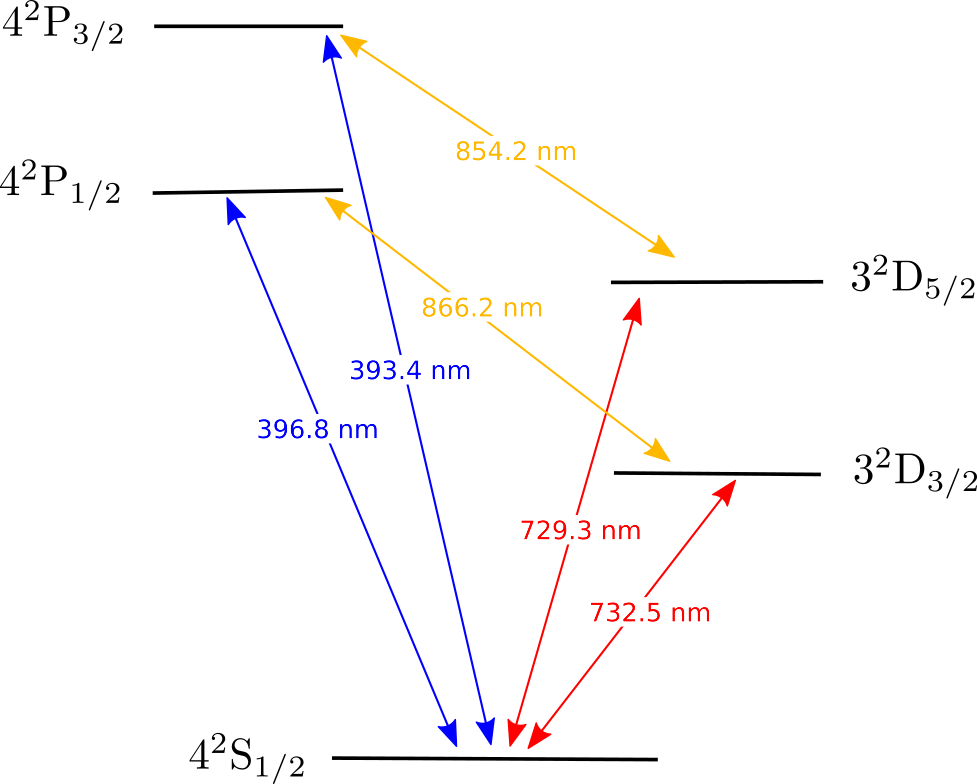
\includegraphics[width = .6 \textwidth]{calciumscheme}
\caption{Level scheme of $^{40}\text{Ca}^+$. Detailed description is in section \ref{sec:calciumion}. For quantum computing purposes, the chosen qubit transition is the long lived quadropole transition $\ket{\text{S}_{1/2}} \to \ket{\text{D}_{5/2}}$ at 729nm.}
\label{qubitschemereference}
\end{figure}

Qubits can be encoded in any pair of orthogonal states. In the case of an ion it is possible to take two internal electronic states, the qubit is then implement in their transition. In figure \ref{qubitschemereference} the level scheme of $^{40}\text{Ca}^+$ is presented. The lifetime of the excited level has to be long enough to carry out all the quantum operation without spontaneous scattering. A common choice is the transition $\ket{\text{S}_{1/2}} \to \ket{\text{D}_{5/2}}$, where the ground state $\ket{\text{S}_{1/2}}$ represents the state $\ket{0}$ and the excited state $\ket{\text{D}_{5/2}}$ will be $\ket{1}$. As these levels are separated by an optical frequency, this kind of qubit is often referred to as optical qubit. Lasers provide a way to directly manipulate the population of the two levels and therefore to manipulate the state of the qubit.\\
The interaction between ion and laser can be understood in terms of a simple model: a two-level atom with dipole interaction with laser field. Consider the system in figure \ref{2levelatom}, where the states $\ket{0}$ and $\ket{1}$ are separated by a frequency $\omega_0$, while the laser is assumed to be monochromatic with frequency $\omega_l$. The difference $\Delta = \omega_l -\omega_0$ is called detuning and we assume to be in the near resonant regime $\Delta \ll \omega_0$. The laser light in this case can be described classicaly in the dipole approximation.
This assumption can be explained as follow, the wavelength of transitions in an atom, are typically in the optical regime: hundreds of nanometers, which is order of magnitude greater then the typical atom dimension. Thus, the electric field can be considered constant over the atom size. This allows to expand the electric field in Taylor series and remove every spatial dependent term in the so called dipole approximation.
\begin{figure}
\centering
\includegraphics[width = .4\textwidth]{2levelatom}
\caption{2-level atom scheme, the ground and excited states are denoted as $\ket{0}$, and $\ket{1}$. $\omega_l$ is the laser frequency, which is detuned by $\Delta \equiv \omega_l - \omega_0$ from the transition frequency $\omega_0$.}
\label{2levelatom}
\end{figure}
The Hamiltonian of the atomic part can be written as:
\begin{equation}
H_a = \hbar\omega_0 \ket{1}\bra{1},
\end{equation}
where $\omega_0$ is the frequency difference between the ground and excited state, the energy of the ground state has also been set to 0. The Hamiltonian of the interaction between the dipole atomic moment $d$ and the electric field of the laser can be written \cite{steck}
\begin{equation}
H_{int} = -d\cdot E
\end{equation}
where the electric field will be treated classically and the dipole approximation is assumed. This means
\begin{equation}
E(t) = \hat{\varepsilon} E_0 \cos(\omega t+\varphi) = \hat{\varepsilon} \frac{E_0}{2} \left(e^{-i(\omega t+\varphi)} + e^{i(\omega t+\varphi)}\right),
\end{equation}
where $\varepsilon$ is a the unit polarization vector. The next step is to work out the dipole operator, this can be done by applying the identity $\ket{0}\bra{0} + \ket{1}\bra{1}$ on both sides of $d$. Due to parity arguments \cite{steck}, only the non diagonal terms are non vanishing, giving
\begin{equation}
d = \braket{0|d|1}\left(\ket{0}\bra{1} + \ket{1}\bra{0}\right) \equiv \braket{0|d|1}(\sigma + \sigma^\dagger).
\end{equation}
Combining the last three equations yields
\begin{equation}
H_{int} = - \braket{0|\hat{\varepsilon} d|1}\frac{E_0}{2}(\sigma e^{i(\omega_l t+\varphi)} + \sigma^\dagger e^{-i(\omega_l t+\varphi)} + \sigma e^{-i(\omega_l t+\varphi)} + \sigma^\dagger e^{i(\omega_l t+\varphi)})
\end{equation}
A rotating wave approximation is used now, essentially $\sigma$ ($\sigma^\dagger$) evolves in time as $\propto e^{-i\omega_0 t}$ ($\propto e^{i\omega_0 t}$), therefore we can drop the fast oscillating terms in the last equation and keeping only those that depends on time as $\propto e^{\pm i(\omega_l-\omega_0 )t}$. The validity of this approximation is given by the facts that $\omega$ and $\omega_0$ are in the optical regime, thus they oscillate extremely fast and average to zero, the interesting slow dynamic is given only by their difference, aka detuning.
With this approximation we arrive at the final form of the interaction Hamiltonian
\begin{equation}
H_{int} = \frac{\hbar \Omega}{2}(\sigma e^{i(\omega_l t+\varphi)} + \sigma^\dagger e^{-i(\omega_l t+\varphi)}),
\end{equation}
 where we defined the Rabi frequency $\Omega \equiv - \braket{0|\hat{\varepsilon} d|1}E_0/\hbar$. The Rabi frequency depends linearly with the applied electrical field and hence its square is proportional to the intensity of the laser $\Omega ^2 \propto I$. To summarize, the final system Hamiltonian is
 \begin{equation}
 \label{2levelatomhamiltonian}
H = H_a + H_{int} = \hbar\omega_0 \ket{1}\bra{1} + \frac{\hbar \Omega}{2}(\sigma e^{i(\omega_l t+\varphi)} + \sigma^\dagger e^{-i(\omega_l t+\varphi)}).
 \end{equation}
This Hamiltonian depends explicitly on time, which could lead to unnecessary complications if we want to solve the dynamics. To eliminate the time dependence, we can go in the rotating frame with the unitary transformation $U = e^{i\omega_l t \ket{1}\bra{1}}$, the Hamiltonian in this frame is
\begin{equation}
\label{Hamiltonianrotatingframe}
\widetilde{H} = -\hbar \Delta \ket{1}\bra{1} + \frac{\hbar \Omega}{2}(e^{i\varphi}\sigma + e^{-i\varphi}\sigma^\dagger)
\end{equation}
The time dependence is now gone, and the unitary evolution matrix can be calculated as
\begin{equation}
\label{laserpulse}
U(t) = \exp\left\{-\frac{i}{\hbar} \widetilde{H} t \right\} =
 \begin{pmatrix}
  \cos\left(\frac{\widetilde{\Omega} t}{2}\right) + i \frac{\Delta}{\widetilde{\Omega}} \sin\left(\frac{\widetilde{\Omega} t}{2}\right) & -ie^{i\varphi}\frac{\Omega}{\widetilde{\Omega}}  \sin\left(\frac{\widetilde{\Omega} t}{2}\right) \\
  -ie^{-i\varphi}\frac{\Omega}{\widetilde{\Omega}}  \sin\left(\frac{\widetilde{\Omega} t}{2}\right)  & \cos\left(\frac{\widetilde{\Omega} t}{2}\right) - i \frac{\Delta}{\widetilde{\Omega}} \sin\left(\frac{\widetilde{\Omega} t}{2}\right)
\end{pmatrix}.
\end{equation}
Where $\widetilde{\Omega} = \sqrt{\Delta^2 + \Omega^2}$ is the generalized Rabi frequency. With this matrix we can calculate all the dynamic we need. In the case of zero detuning $\Delta = 0$, we also notice that the matrix is the same as equation \eqref{quantumgates}. Thus, a resonant laser pulse implements the qubit rotation $U_{\varphi}(\theta)$, the rotation around the z axis is performed with a laser pulse as well, but far detuned from the transition. We will explore this possibility later in the AC Stark shift.\\
As example, let us take the atom in the ground state $\ket{\psi} = \ket{0}$ and apply the unitary evolution \eqref{laserpulse}. The probability to be in the excited state becomes
\begin{equation}
\mathbb{P}\{\ket{1}\}(t) = |\braket{1|U(t)|0}|^2 = \frac{\Omega^2}{\Omega^2+\Delta^2} \sin^2\left(\frac{\widetilde{\Omega}t}{2} \right)
\end{equation}
This equation is plotted in figure \ref{rabiflops}. For $\Delta = 0$, we get a cosine behaviour, the so called Rabi oscillations. The probability amplitude for the electron, under continuous drive by a laser, will oscillate between the ground and excited state at a frequency $\Omega$. Detuning damps the amplitude of such oscillations and increases the oscillation frequency. Rabi oscillations are an important tool in quantum information, laser pulses can prepare the state of the qubit in any superposition, e.g. starting in the $\ket{0}$ state, a $\pi/2$ pulse ($\Omega t = \pi/2$ and phase $\varphi=0$) will result in the state $(\ket{0} - i\ket{1})/\sqrt{2}$, with a $\pi$ pulse ($\Omega t = \pi$, $\varphi=\pi$) the population is completely transferred to another level $\ket{0}\to \ket{1}$. These pulses can be used to implement the Hadamard gate of equation \eqref{Hadamard}.
\begin{figure}[H]
\centering
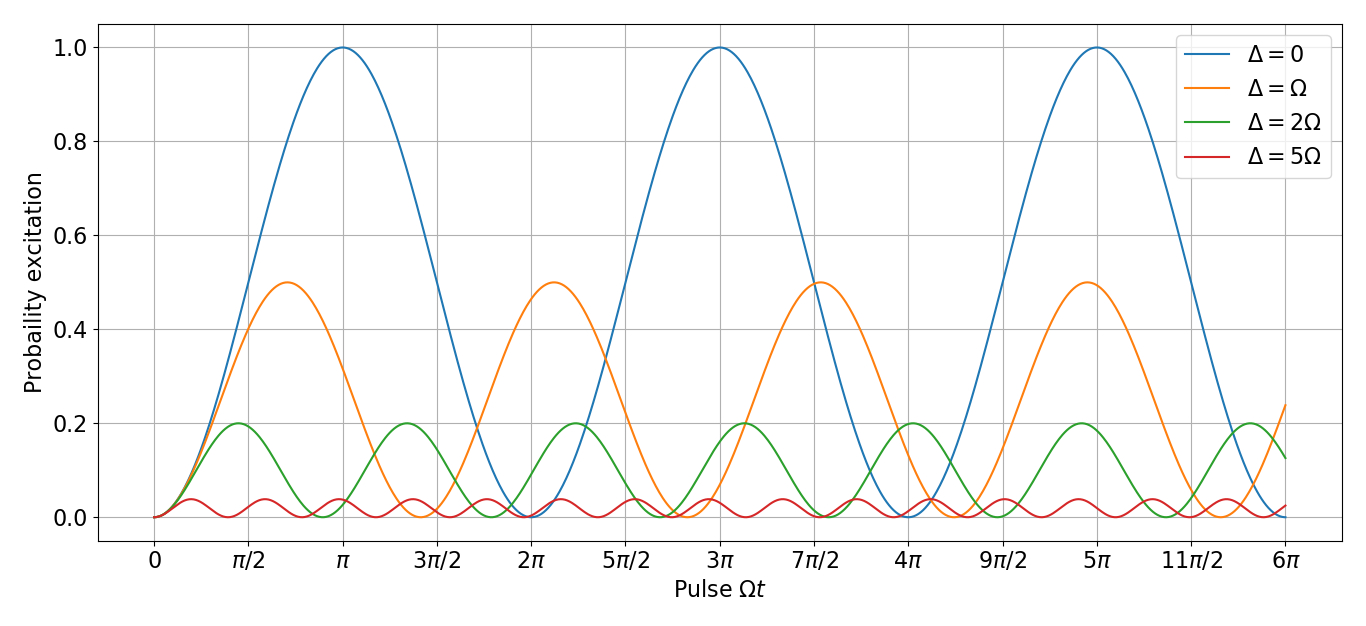
\includegraphics[width = 1\textwidth]{rabiflops}
\caption{Rabi flops for different detuning $\Delta$}
\label{rabiflops}
\end{figure}
As the light is detuned from the transition, Rabi oscillations are suppressed: the amplitude is reduced by a factor of 0.5 already with $\Delta = \Omega$, while a factor of 10 in reduction is achieved with a detuning of $\Delta/\Omega = 5$. However, another effect persists in the off-resonant regime: the energy levels are shifted.
The shift $\delta$ can be calculated by finding the eigenvalues of the Hamiltonian \eqref{Hamiltonianrotatingframe}, which can be written in matrix form and diagonalized. We find that there are two eigenstates $\ket{+}$ and $\ket{-}$ called dressed states with eigenvalues
\begin{equation}
E_{\pm} = -\frac{\hbar\Delta}{2} \pm \frac{\hbar}{2}\sqrt{\Delta^2 +\Omega^2}.
\end{equation}
In the limit $\Delta \gg \Omega$, dressed states tend to the bare states $\ket{+} \to \ket{1},\ket{-}\to \ket{0}$, and the energies becomes
\begin{equation}
\label{eq:starkshift}
E_{\pm} \to -\frac{\hbar \Omega}{2} \pm \frac{\hbar \Omega}{2} \pm \frac{\hbar \Omega^2}{4\Delta} \implies \delta = \pm\frac{\Omega^2}{4\Delta}.
\end{equation}
The effective Hamiltonian for the off-resonant regime can be derived following a Markovian approximation \cite{acstarkhamiltonian}
\begin{equation}
H_{AC} = \frac{1}{\hbar \Delta} [\sigma,\sigma^\dagger] = \frac{\hbar \delta}{2}\sigma_z
\end{equation}
The corresponding evolution is
\begin{equation}
\label{acstarkrotation}
U(t) = \exp\left\{-\frac{i}{\hbar} H_{AC} t \right\} =
 \begin{pmatrix}
   \exp\left\{i\frac{\delta}{2}t\right\} & 0\\
   0 & \exp\left\{i\frac{\delta}{2}t\right\}
\end{pmatrix}.
\end{equation}
This matrix implements the quantum gate from equation \eqref{quantumgates}. Furthermore, Ac Stark shift can also implement the phase gate $R_{\phi}$ of equation \eqref{Hadamard}, but it requires a third energy level.
\subsubsection{Three-level model}
\label{sec:threelevel}
\begin{figure}
\centering
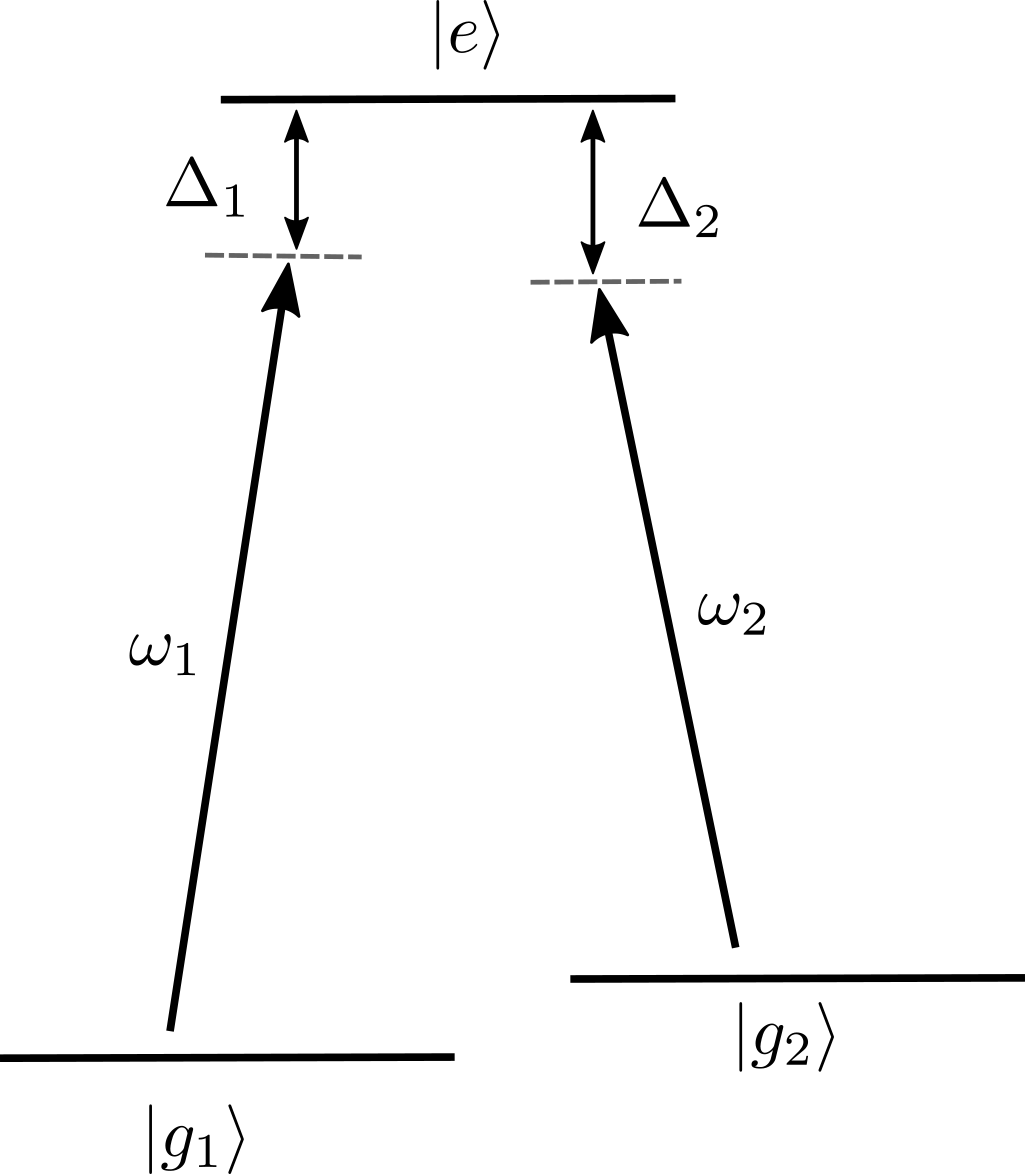
\includegraphics[width = .3\textwidth]{3levelmodel}
\caption{3 level atom model. Two long lived ground states $\ket{g_1}$, $\ket{g_2}$ couple to an excited level $\ket{e}$ through two laser of frequencies $\omega_1$, $\omega_2$ detuned respectively $\Delta_1,\Delta_2$ from the transition.}
\label{3levelmodel}
\end{figure}
We extend our model to a 3 level $\Lambda$ type atom, which closer resemble the real experimental system, driven by two lasers. The model is more complex but contains new effects that explain photon generation and qubit gates. In particular, stimulated Raman transition will be discussed, and we will show how, under certain conditions, the system can be approximated as an effective 2 level atom. The system is depicted in figure \ref{3levelmodel}, two ground states $\ket{g_1}$ and $\ket{g_2}$ are present together with a common excited state $\ket{e}$. Two different lasers drive the transition $\ket{g_1} \to \ket{e}$ and $\ket{g_2} \to \ket{e}$ with detuning $\Delta_1$ and $\Delta_2$. In the case of calcium, the ground states are $\ket{\text{S}_{1/2}}$, and $\ket{\text{D}_{5/2}}$. This is the qubit transition, and it is long lived, such that any spontaneous emission between S and P can be neglected. The excited level is $\ket{\text{P}_{3/2}}$ which can decay into both ground states.\\
In this model we assume that the two ground states are not separated by an optical frequency $\omega_{02} - \omega_{01} \ll \omega_1,\omega_2$, and that the detunings are nearly equal $\Delta_1 \simeq \Delta_2$. As a consequence, each laser light couples only to one transition.\\
The mathematical description is similar to the one described in section \ref{laserioninteractions} for the 2 level atom with the addition of extra terms. The bare atom Hamiltonian is
\begin{equation}
H_a = -\hbar \omega_{01}\ket{g_1}\bra{g_1} - \hbar \omega_{02}\ket{g_2}\bra{g_2},
\end{equation}
with the convention of setting the excited level energy to 0. The electric field is now the sum of the two lasers lights
\begin{equation}
E(t) = \hat{\varepsilon_{01}} E_{01} \cos(\omega_{1} t \varphi_1) + \hat{\varepsilon_{02}} E_{02} \cos(\omega_2 t + \varphi_2).
\end{equation}
We still apply the dipole and the rotating wave approximation to the interaction between electric field and atom. Finally transforming into the rotating frame gives the full final Hamiltonian as \cite{steck}
\begin{equation}
H = \hbar \Delta_1 \ket{g_1}\bra{g_1} + \hbar\Delta_2 \ket{g_2}\bra{g_2}+ \frac{\hbar \Omega_1}{2}\left(\sigma_1 e^{i\varphi_1} +\sigma_1^\dagger e^{i\varphi_1}\right)+ \frac{\hbar \Omega_2}{2}\left(\sigma_2 e^{i\varphi_2} +\sigma_2^\dagger e^{i\varphi_2}\right),
\end{equation}
where $\Omega_i = -\frac{\braket{g_1|\varepsilon_i \cdot d|e}E_{i}}{\hbar}$, and $\sigma_i = \ket{g_i}\bra{e}$. This Hamiltonian describes a Raman process, state population can be transferred coherently from $g_{1}$ to $g_{2}$, without exciting to the $\ket{e}$ level. This happens at the Raman resonance $\Delta_1 = \Delta_2 \equiv \Delta$ if the detuning is large enough to eliminate adiabatically population in the $\ket{e}$ level, i.e. $\Delta \gg \Omega_1,\Omega_2$. Intuitively, this corresponds to the situation where the difference of the two driving frequencies $(\omega_1-\omega_2)$ is equal to the frequency splitting between $\ket{g_1}$, and $\ket{g_2}$.\\
As the excited level is eliminated, it can be showed \cite{russo} that the dynamics can be described from an effective 2 level system equivalent of that described in section \ref{laserioninteractions}. The effective Rabi frequency can be written as
\begin{equation}
\Omega_{eff} = \frac{\Omega_1\Omega_2}{2\Delta}.
\end{equation}


\subsubsection{Dissipative processes}
\label{sec:dissipation}
In the previous treatments we neglected dissipative processes as spontaneous emission to simplify the mathematical description. However, dissipative processes can play a role and it is important to understand them. In this section we will focus exclusively on spontaneous emission, later cavity decay will also be introduced.\\
Dissipative process do not follow an Hermitian evolution, hence their mathematical description is done heuristically by adding terms in the Heisenberg equation
\begin{equation}
\label{masterequation}
\frac{d\rho}{dt} = \frac{1}{i\hbar}[H,\rho] + \mathcal{L}(\rho).
\end{equation}
This equation is usually referred to as master equation in Lindblad form, where $\rho$ is the density matrix of system. The superoperator
$\mathcal{L}(\rho)$ contains phenomena not included in the Hamiltonian. For spontaneous emission, the form of $\mathcal{L}(\rho)$ is \cite{quantumnoise}
\begin{equation}
\mathcal{L}(\rho) = \frac{\Gamma}{2}(2\sigma \rho \sigma^\dagger -\sigma^\dagger\sigma \rho - \rho \sigma^\dagger \sigma),
\end{equation}
where $\Gamma$ is the decay rate. $\Gamma$ represents the coupling between atom and environment, and can be calculated from Fermi's golden rule \cite{doi:10.1142/p941}
\begin{equation}
\Gamma = \frac{\omega_0^3 |d|^2}{3\pi\varepsilon_0 \hbar c^3}.
\end{equation}
The master equation \eqref{masterequation} can be explicitly written for every component of the density matrix $\rho$,
in the rotating frame they are called optical Bloch equations. The solution for the excited population in the case of the 2 level atoms shows that the effect of spontaneous decay is to damp Rabi oscillations. In this case, on long time scale population exchange is suppressed, as it reaches a steady state. This regime is presented is section \ref{sec:doppler_cooling}.\\
In the case of the three level model, the excited level $\ket{e}$ can decay to both ground states with rates $\Gamma_{g_1}$, and $\Gamma_{g_2}$. We are most interested in the decay rate $\Gamma_{g_1} \def \Gamma$ from $\ket{e}\to\ket{g_1}$ as the other transition in calcium is often repumped. In this case, in the effective 2 level system picture, the spontaneous emission is modified as \cite{russo}
\begin{equation}
\Gamma_{eff} = \left(\frac{\Omega_1}{2 \Delta_1}\right)^2 \cdot \Gamma.
\end{equation}
The ratio between this result and the Ac Stark shift \eqref{eq:starkshift} $\delta/\Gamma_{eff}\propto \Delta$ dictates which effect is dominant, i.e. spontaneous scattering can be eliminated leaving only Stark shift as effect depending on the detuning.




\section{Quantum networking with trapped ions}
\subsection{General introduction}
A quantum network is a collection of quantum processors, denominated nodes, interconnected with quantum channels. Quantum channels have the unique property to be able to transmit quantum state among the nodes and distribute entanglement over the network \cite{kimble}. There are two classes of quantum networks which are differentiated by the purpose, networks can be used for transmission of information, i.e. communication, or for distributed quantum computation, i.e. scaling of quantum processors \cite{ion_quantumnetwork}.
In these two cases the topology of the network is different, but the core elements are the same: a node, where quantum information is prepared, manipulated, and stored; and a link that connects nodes. Links can be realized in free space \cite{Hughes2002} or with optical fibers, photons can carry quantum information over long distance with high speed. Nodes can be realized using different physical systems: trapped ions \cite{ion_quantumnetwork}, neutral atoms \cite{Ritter2012}, atomic ensembles \cite{kimble}. Nodes and links are connected through an interface that converts a stationary qubit in a node to a flying qubit over the network.  In the next section we will explore how an interface can be realized by placing an ion based quantum memory in an optical cavity.\\
For a fully deployed quantum network, many challenges have to be faced. Faithful transmission of a quantum states over long distances can be a daunting problem as quantum information cannot be cloned \cite{nocloning}, and noisy channels can destroy the delicate nature of qubits. Quantum repeaters have been designed \cite{quantumrepeters} to circumvent these problems through a series of protocols which includes error corrections, or entanglement purification \cite{Pan2001}. More protocols are also available to  entangle qubits located in spatially separated quantum nodes \cite{Duan2001}. Once entanglement has been established between nodes, other network functionalities become available, like for instance teleportation \cite{PhysRevLett.70.1895}. Entanglement generation, and quantum repeaters are just some examples of the fundamental steps necessary for building a quantum network, for a more in depth review look at \cite{Wehnereaam9288}.


\subsection{Cavity QED}
Trapped ions can become quantum nodes of a quantum network by placing them in a cavity. Ions emits photon by spontaneous emission, or stimulated emission. The problem with spontaneous emission is that the photonic channel of emission is random and in free space. To realize a quantum interface, photon should be produces almost deterministically in defined mode. The trick is to use a cavity tuned to one particular transition, such that the probability of a photon to be emitted in the cavity mode is greatly enhanced. In this section we describe a simple model of a two-level system in a cavity, the derivation is similar to section \ref{laserioninteractions}, with the difference that in a cavity the electric field is quantized. Using the mode operator $a,a^\dagger$ the electric field inside a cavity can be written as:
\begin{equation}
E = A(f(r)a + f^*(r)a^\dagger)
\end{equation}
where $A$ is an amplitude, and $f(r)$ is the spatial mode profile \cite{helene}. The interaction between he field and the cavity is obtained as from $H_{int} = -d\cdot E$, following a rotating wave approximation the result is
\begin{equation}
H_{int} = \hbar g (\sigma a^\dagger + \sigma^\dagger a),
\end{equation}
where $g = A \braket{g|d|e} f(r)$ is called cavity coupling constant. It is analogous to the Rabi frequency, it gives an idea of the coupling between the cavity field and the 2-level atom. An important dependence of $g$ can be found by considering that $f(r)$ is inversely proportional to the volume of the cavity $V$, i.e.
\begin{equation}
g \propto \braket{g|d|e} \sqrt{\frac{\omega}{2\varepsilon_0 \hbar V}}.
\end{equation}
The coupling therefore, increases with decreasing cavity volume and viceversa.\\
The total system Hamiltonian includes also the atomic part, and a single mode optical field. It takes the name of Jaynes-Cummings Hamiltonian and it is written as \cite{qedreview}
\begin{equation}
H = \hbar \omega_0 \ket{1}\bra{1} + \hbar \omega a^\dagger a + \hbar g (\sigma a^\dagger + \sigma^\dagger a).
\end{equation}
States now are a product state of the atomic part and the photon number $\ket{g,n},\ket{e,n}$. They are however not the eigenstates of the Jaynes-Cumming Hamiltonian. It can be seen that this Hamiltonian is block diagonal, which means that each $2\times 2$ block can be diagonalized, the dressed states found after diagonalization are similar to the semiclassical model. Moreover, also the dynamics is analogue to the semiclassical case, Rabi oscillations are still present with quantized Rabi frequency given by $\Omega_n = \sqrt{4(n+1)g^2 +\Delta^2}$.\\
The presence of a cavity makes dynamics more interesting, especially when considering spontaneous emission and interaction with cavity modes. For a mathematical description, we need to introduce dissipative process that do not follow an Hermitian evolution. This is done heuristically by adding terms in the Heisenberg equation
\begin{equation}
\label{masterequation}
\frac{d\rho}{dt} = \frac{1}{i\hbar}[H,\rho] + \mathcal{L}(\rho).
\end{equation}
This equation is usually referred to as master equation in Lindblad form, where $\rho$ is the density matrix of system. The superoperator
$\mathcal{L}(\rho)$ contains phenomena not included in the Hamiltonian. In our case, we are most interested in two process: spontaneous emission in a free space field mode, and decay in one cavity mode and out of the cavity. The first is quantified with the decay rate $\Gamma$, while the latter is characterized by the decay rate $\kappa$. The functional dependence of these two terms goes as \cite{steck}
\begin{equation}
\mathcal{L}(\rho) = \Gamma\mathcal{D}(\sigma)\rho + \kappa \mathcal{D}(a)\rho.
\end{equation}
A good approximation of the model is given in the \emph{strong coupling} regime $g\ll \Gamma,\kappa$, where damping due to dissipative process is slow and dynamics is mainly driven coherently by the coupling atom-cavity $g$. The decay rate $\kappa$ depends exclusively on the cavity parameters as \cite{helene}
\begin{equation}
\kappa =\frac{c\pi}{FL},
\end{equation}
where $F$ is the cavity finesse, and $L$ the length. In the design of the experiment one must play and compromise with these three parameters in order to reach a good coupling ion-cavity but also being able to send photons out of the cavity.

\subsection{Photon generation}
\label{sec:ramanprocess}
By placing a cavity around the trap, photon generation is enabled. The cavity mediated Raman process is responsible for this phenomenon. It can be explained strating from a three level atom like in figure \ref{ramanprocess}. The electron is initially in the ground state $\ket{0}$, a laser pulse excite the transition $\text{S}_{1/2} \to \text{D}_{3/2}$ detuned properly to eliminate the population in the $\ket{1}$ level. Among the decay channels of the electron, the decay $\text{P}_{3/2} \to \text{D}_{5/2}$ is enhanced due to the presence of the cavity and therefore the coupling $g$ between the ion and the cavity mode. The electron will more likely decay
to the $\text{D}_{5/2}$ state emitting a photon inside the cavity. Thus the process can be described as $\ket{0}_i\ket{0}_p \to \ket{1}_i\ket{1}_p$ where the subscript $i$ indicates the ion and $p$ the photon number in the cavity. The detuning is set such as $\Delta \gg \Omega,g$, in this regime the whole process can be described as a single transition with effective Rabi frequency of \cite{helene}
\begin{equation}
\label{omegaeff}
\Omega_{eff} = \frac{\Omega g}{2\Delta}.
\end{equation}
It is equivalent of a classical Raman process driven with two laser pulses on the two different transitions, but in this case the second laser is substituted by the vacuum standing wave of the cavity. In order to avoid decay in other channels, one must be sure that $\Omega_{eff}$ is larger than the effective decay rate of other spontaneous emission $\Omega_{eff}\gg \Gamma_{eff}$. Moreover, the photon should leave the cavity after the transfer is complete, this is ensured by $\Omega_{eff} >\kappa$.\\
In the real case the electronic states are also shifted due to a magnetic field generated by a permanent magnet perpendicular to the cavity axis and at $45^{\circ}$ with respect to the trap axis. This is done in the optics of achieving ion-photon entanglement, since in that case multiple Zeeman levels should be addressed. The situation is therefore further complicated and the polarization of the laser field should be taken into consideration. In figure (), the Zeeman structure of $^{40}\text{Ca}^+$ is depicted. One can start from the state $\ket{\text{S}_{1/2},m_j = -1/2}$. From here three choices of polarization can be taken: $\sigma^-,\pi,\sigma^+$, for each choice three Raman transition are possible, the most favorable in the case of the magnetic field orthogonal to the cavity axis is \cite{stuteinterface}
\begin{equation}
\ket{\text{S}_{1/2},-1/2}\to\ket{\text{P}_{3/2},-3/2} \to \ket{\text{D}_{5/2},-5/2}.
\end{equation}
In this case the transitions strengths, i.e. the projection on the laser polarization onto the dipole moment, and the same projection onto the cavity axis are maximized.\\
The generated photon from this process can be entangled with the ion state by driving this Raman transition with a bichromatic beam. This means that the laser pulse drives two transitions at the same time, for example the one that ends up in $\ket{\text{D}_{5/2},-5/2}$ and $\ket{\text{D}_{5/2},-3/2}$. In this instance, the generated photon will be a superposition of $\sigma^+$ and $\pi$ polarization. With respect to the cavity it means vertical and horizontal polarization. The final state of the bichromatic transition is therefore
\begin{equation}
\ket{\psi} = \ket{\text{D}_{5/2},-5/2}\ket{H} + \ket{\text{D}_{5/2},-3/2}\ket{V}.
\end{equation}
In the real experiment the designed cavity is near concentric with a length of $19.9$ mm, and radii of curvature of $9.98$ mm. The cavity length is actively stabilized with a PDH type feedback which locks the mirrors position to a 806nm laser. One mirror of the cavity is highly reflective $T_1 = 2.2$ ppm, while the other is more transmissive $T_2 = 97$. This asymmetry of the mirrors allows for the produced photons to exit one from one side in most cases and subsequently coupled to a fiber. The probability to get a photon out of the cavity from the designed mirror can be determined from the transmission and losses of the cavity, the maximum achievable is $P_{max} = 0.83$. The maximum $g$ factor achievable with this geometry is $g = 2\pi \times 1.53$ MHz.
\begin{figure}[H]
     \centering
     \begin{subfigure}[b]{0.49\textwidth}
         \centering
         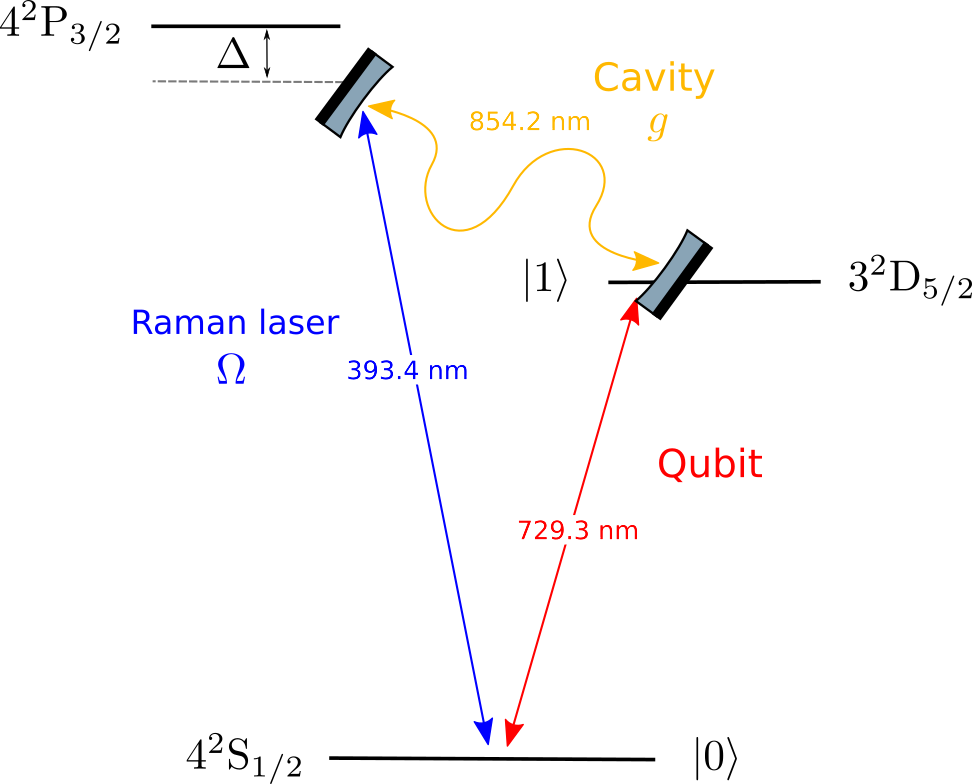
\includegraphics[width=\textwidth]{ramanprocess}
         \caption{Diagram for the Raman transition. A pulse at 393nm triggers the generation of a 854nm photon inside a the cavity. In the process the ion gets excited to the $\ket{1}$ level.}
     \end{subfigure}
     \hfill
     \begin{subfigure}[b]{0.49\textwidth}
         \centering
         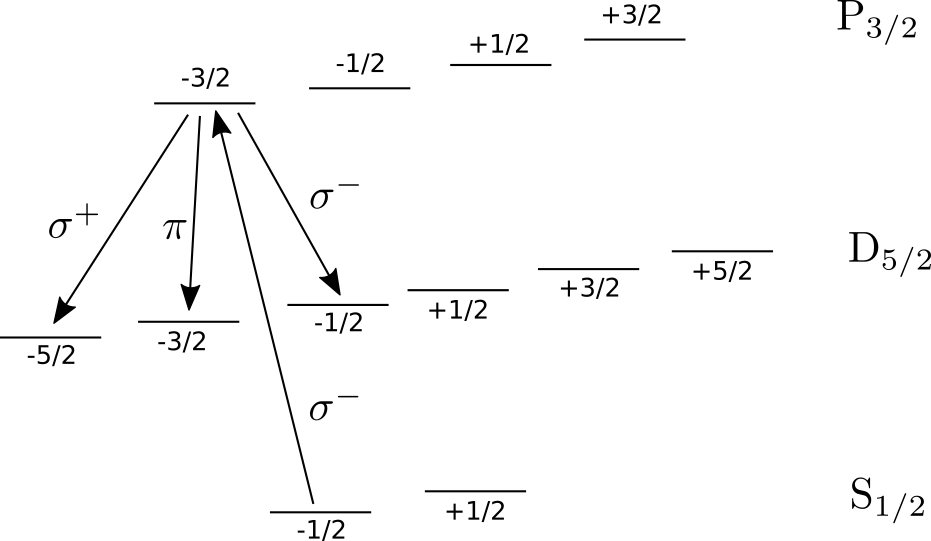
\includegraphics[width=\textwidth]{zeemanstructure}
         \caption{Zeeman structure of the relevant levels for the Raman process.}
         %\label{fig:three sin x}
         \vspace{1em}
     \end{subfigure}
        \caption{}
      \label{ramanprocess}
      %  \label{fig:three graphs}
\end{figure}
 The Finesse of the cavity for the TEM$_{00}$ mode is 54000. The other cavity parameters are $\kappa = 2\pi \times 70$ kHz, and $\gamma = 2\pi\times 11.45$ MHz for the $\text{P}_{3/2}$ state. With these numbers the preferred strong regime is not reached, but nonetheless,  it is still possible to produce photons and collect them out of the cavity.

\section{Basics of ion trapping}
\subsection{Linear Paul trap}
Ions are particles that carry an electric charge, therefore electric fields can be used to control ions and ultimately trap them. In order to achieve confinement in 3 dimensions, a 3D potential $\phi(x,y,z)$ with minima in all directions is needed. However, it follows directly from Maxwell equation $\nabla^2 \phi = 0$ that the potential must be antitrapping at least in one direction. There are two workarounds for this problem: the first one introduces magnetic fields to trap particles in some directions, this takes the name of Penning trap \cite{RevModPhys.58.233}. The second solution is the so called Paul trap, and it is what we are going to describe in this section. The idea is to introduce a time varying potential, such that the antitrapping direction is constantly switching between two different dimension. The particles will therefore experience an effective confinement in all direction if the switching is faster compared to the time it takes the particle to respond.\\
The shape of the trap can be adapted to load more ions in different geometries. In our work we utilize a linear Paul trap, which is elongated in one direction. The confinement in this direction is weaker and thus loaded ions will align in a single long string. This kind of trap is depicted in figure \ref{trap}.
\begin{figure}[H]
\centering
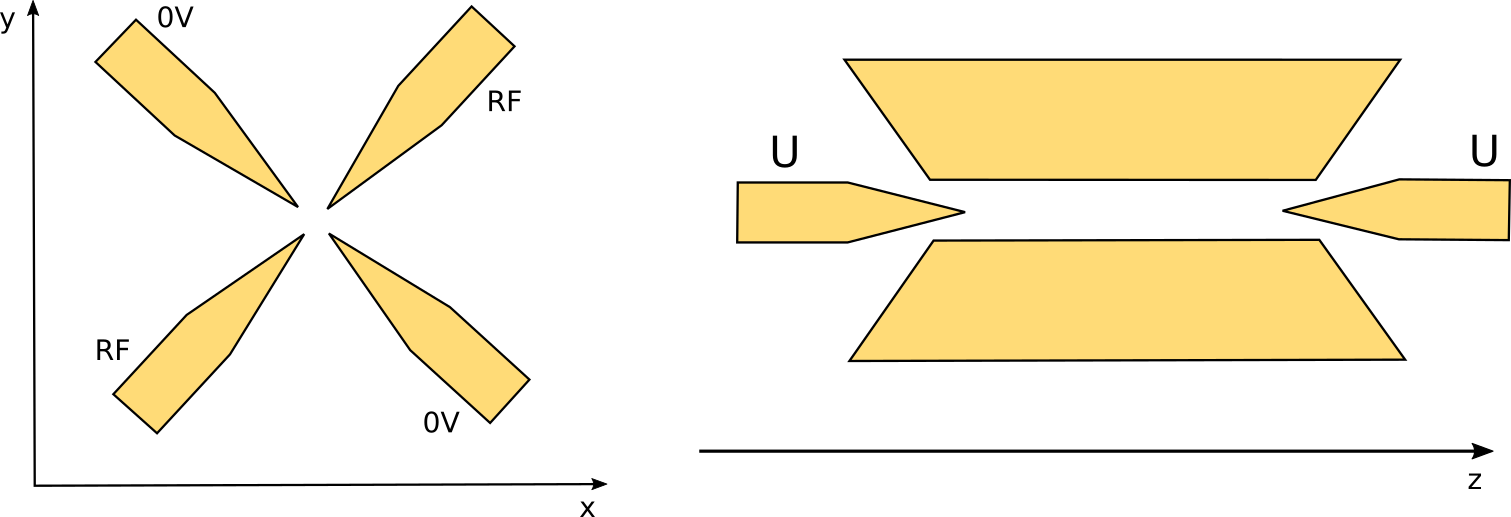
\includegraphics[width = .7\textwidth]{trap}
\caption{A linear paul trap. U is the voltage applied to the electrodes trapping in the $z$ direction, while in the $x-y$ plane trapping is achieved with a radio frequency signal. $r_0$ is the distance from the central axis to the RF electrodes.}
\label{trap}
\end{figure}
The confinement in the $x-y$ plane is provided by 4 electrodes, two of which are grounded and the other two are connected to a radio frequency source. This design is similar to a mass filter, with the difference of additional endcaps electrodes in the $z$ direction that plug the trap and confine also in the axial direction.\\
The potential inside the trap can be described for the $x-y$ plan independently from the $z$ direction. In the case of a linear Paul trap the radial potential is \cite{traptheory}:
\begin{equation}
\phi  = \frac{\Phi_0}{2r_0^2}\left(x^2 - y^2\right),
\end{equation}
where $r_0$ is the distance from the center of the trap to the electrodes. The amplitude consists of a static part $U_0$ and a dynamical one $\Phi_0 = U_0 + V \cos(\Omega_{RF} t)$.
The study of the particle's motion with mass $m$ and charge $e$ inside the trap can be done with classical physics, Newton's second law in this case is
\begin{equation}
m\ddot{x} = -q \frac{\partial \phi}{\partial x} = - \frac{ex}{r_0^2}\left(U_0 + V \cos(\Omega_{RF} t) \right),
\end{equation}
and similarly for $\ddot{y}$. This equation can be written in the form of Mathieu equation \cite{Richards1983} by defining two parameters:
\begin{equation}
a_x = \frac{4eU_0}{\Omega_{RF}^2r_0^2m}, \quad q_x = \frac{2eV}{\Omega_{RF}^2r_0^2m} \implies \ddot{x} +\frac{\Omega_{RF}}{4} \left(a_x + 2q_x \cos(\Omega_{RF} t )\right)x = 0
\end{equation}
and with a change of variable $\tau = \frac{\Omega_{RF} t}{2}$ we end up with
\begin{equation}
\label{mathieu}
\frac{\partial^2 x}{\partial \tau^2}+\left(a_x + 2q_x \cos(2\tau)\right)x = 0
\end{equation}
This kind of equations have stable solutions that can be found in a recursive way with Floquet theorem \cite{iondynamic}. In the limit $a_x \ll q_x \ll 1$, solutions to \eqref{mathieu} are found to be
\begin{equation}
x(t) = x_0 \cos(\omega_x t +\phi_x)\left[1 + \frac{q_x}{2}\cos(\Omega_{RF} t) \right].
\end{equation}
Here, we recognize a slowly varying oscillation $\omega_x$, referred to as \emph{secular motion}, with amplitude modulated by a faster oscillation $\Omega_{RF}$, called \emph{micromotion}. The approximation, named secular, is valid only in the case $\omega_x \ll \Omega_{RF}$. The behaviour of micromotion is dictated by the force due to the potential at the position $\bar{x}$, and the secular motion will follow a time average of the potential $\langle \phi(t) \rangle$. The frequency $\omega_x$ is given in the solution as
\begin{equation}
\label{eq:wx}
\omega_x = \frac{\Omega_{RF}}{2}\sqrt{a_x + \frac{q_x^2}{2}}.
\end{equation}
By imposing real solutions to \eqref{eq:wx}, the stability diagram of the trap can be found. The other spatial dimension can be treated in the same way and the results are the same.\\
Confinement in the axial direction $z$ is purposely weaker, and ions will align in this direction. Two electrodes with constant potential $U$ are present, they create a harmonic potential
\begin{equation}
V = \frac{1}{2}m\omega_z^2z^2,
\end{equation}
where $\omega_z$ is the axial trap frequency. In the case of a string of ions, mutual repulsions must also be included, in the next section we will consider this case.

\subsection{Ion strings}
\label{ionstrings}
For the goals of this thesis, we are interested in the separation between $N$ ions loaded in the trap. This will give us an idea of how narrowly the beam should be focused and will set an appropriate problem spatial scale.\\
Let us consider the $z$ direction where the ions are more weakly confined such that they form a string. The potential can be approximated as harmonic and hence given by
\begin{equation}
V = \sum_{i=0}^N \frac{1}{2}m\omega^2z_i^2 + \sum_{i\neq j}^N\frac{Z^2e^2}{8\pi \epsilon_0}\frac{1}{|z_i-z_j|},
\end{equation}
where $z_i$ is the position of the $i-$th ion, and $Z$ the degree of ionization of the ions. The equilibrium positions can be found at the minima of the potential, i.e. where the first derivative zeros
\begin{equation}
\frac{\partial V}{\partial z_i} = 0 \implies u_i - \sum_{j=1}^{i-1} \frac{1}{(u_i-u_j)^2} + \sum_{j= i+1}^{N} \frac{1}{(u_i-u_j)^2}= 0,
\end{equation}
where we defined the dimensionless quantity $u_i = z_i/l$ and $l^3 = \displaystyle\frac{Z^2 e^2 }{4\pi \epsilon_0 m\omega^2}$.
The last equations can be solved analytically for 2 or 3 ions \cite{ion_spacing}. For the case $N=2$ we get the system
\begin{equation}
\begin{cases}
  u_1 + \frac{1}{(u_1-u_2)^2} = 0\\
  u_2 - \frac{1}{(u_1-u_2)^2} = 0
  \end{cases} \quad \implies \quad u_1 = -u_2,\quad  u_1 = \left(\frac{1}{2}\right)^{2/3} \simeq 0.629
\end{equation}
For $^{40}\text{Ca}^+$ ions (atomic mass $39.96259098(22)$ u \cite{AUDI2003337}) in a Paul trap with axial confinement of $\omega_z = 2\pi \times 1$ MHz, we have $l \simeq 4.45\times 10^{-6}\,$m, which means that 2 ions are separated by $\simeq 5.6\, \mu$m. This size is accessible since it is above diffraction limit for optical atomic transitions.
In figure \ref{positions_ions} ions positions are presented for different number of ions $N$ trapped with an axial confinement of $\omega_z = 2\pi \times 1$ MHz.

\begin{figure}[H]
\hspace{-5em}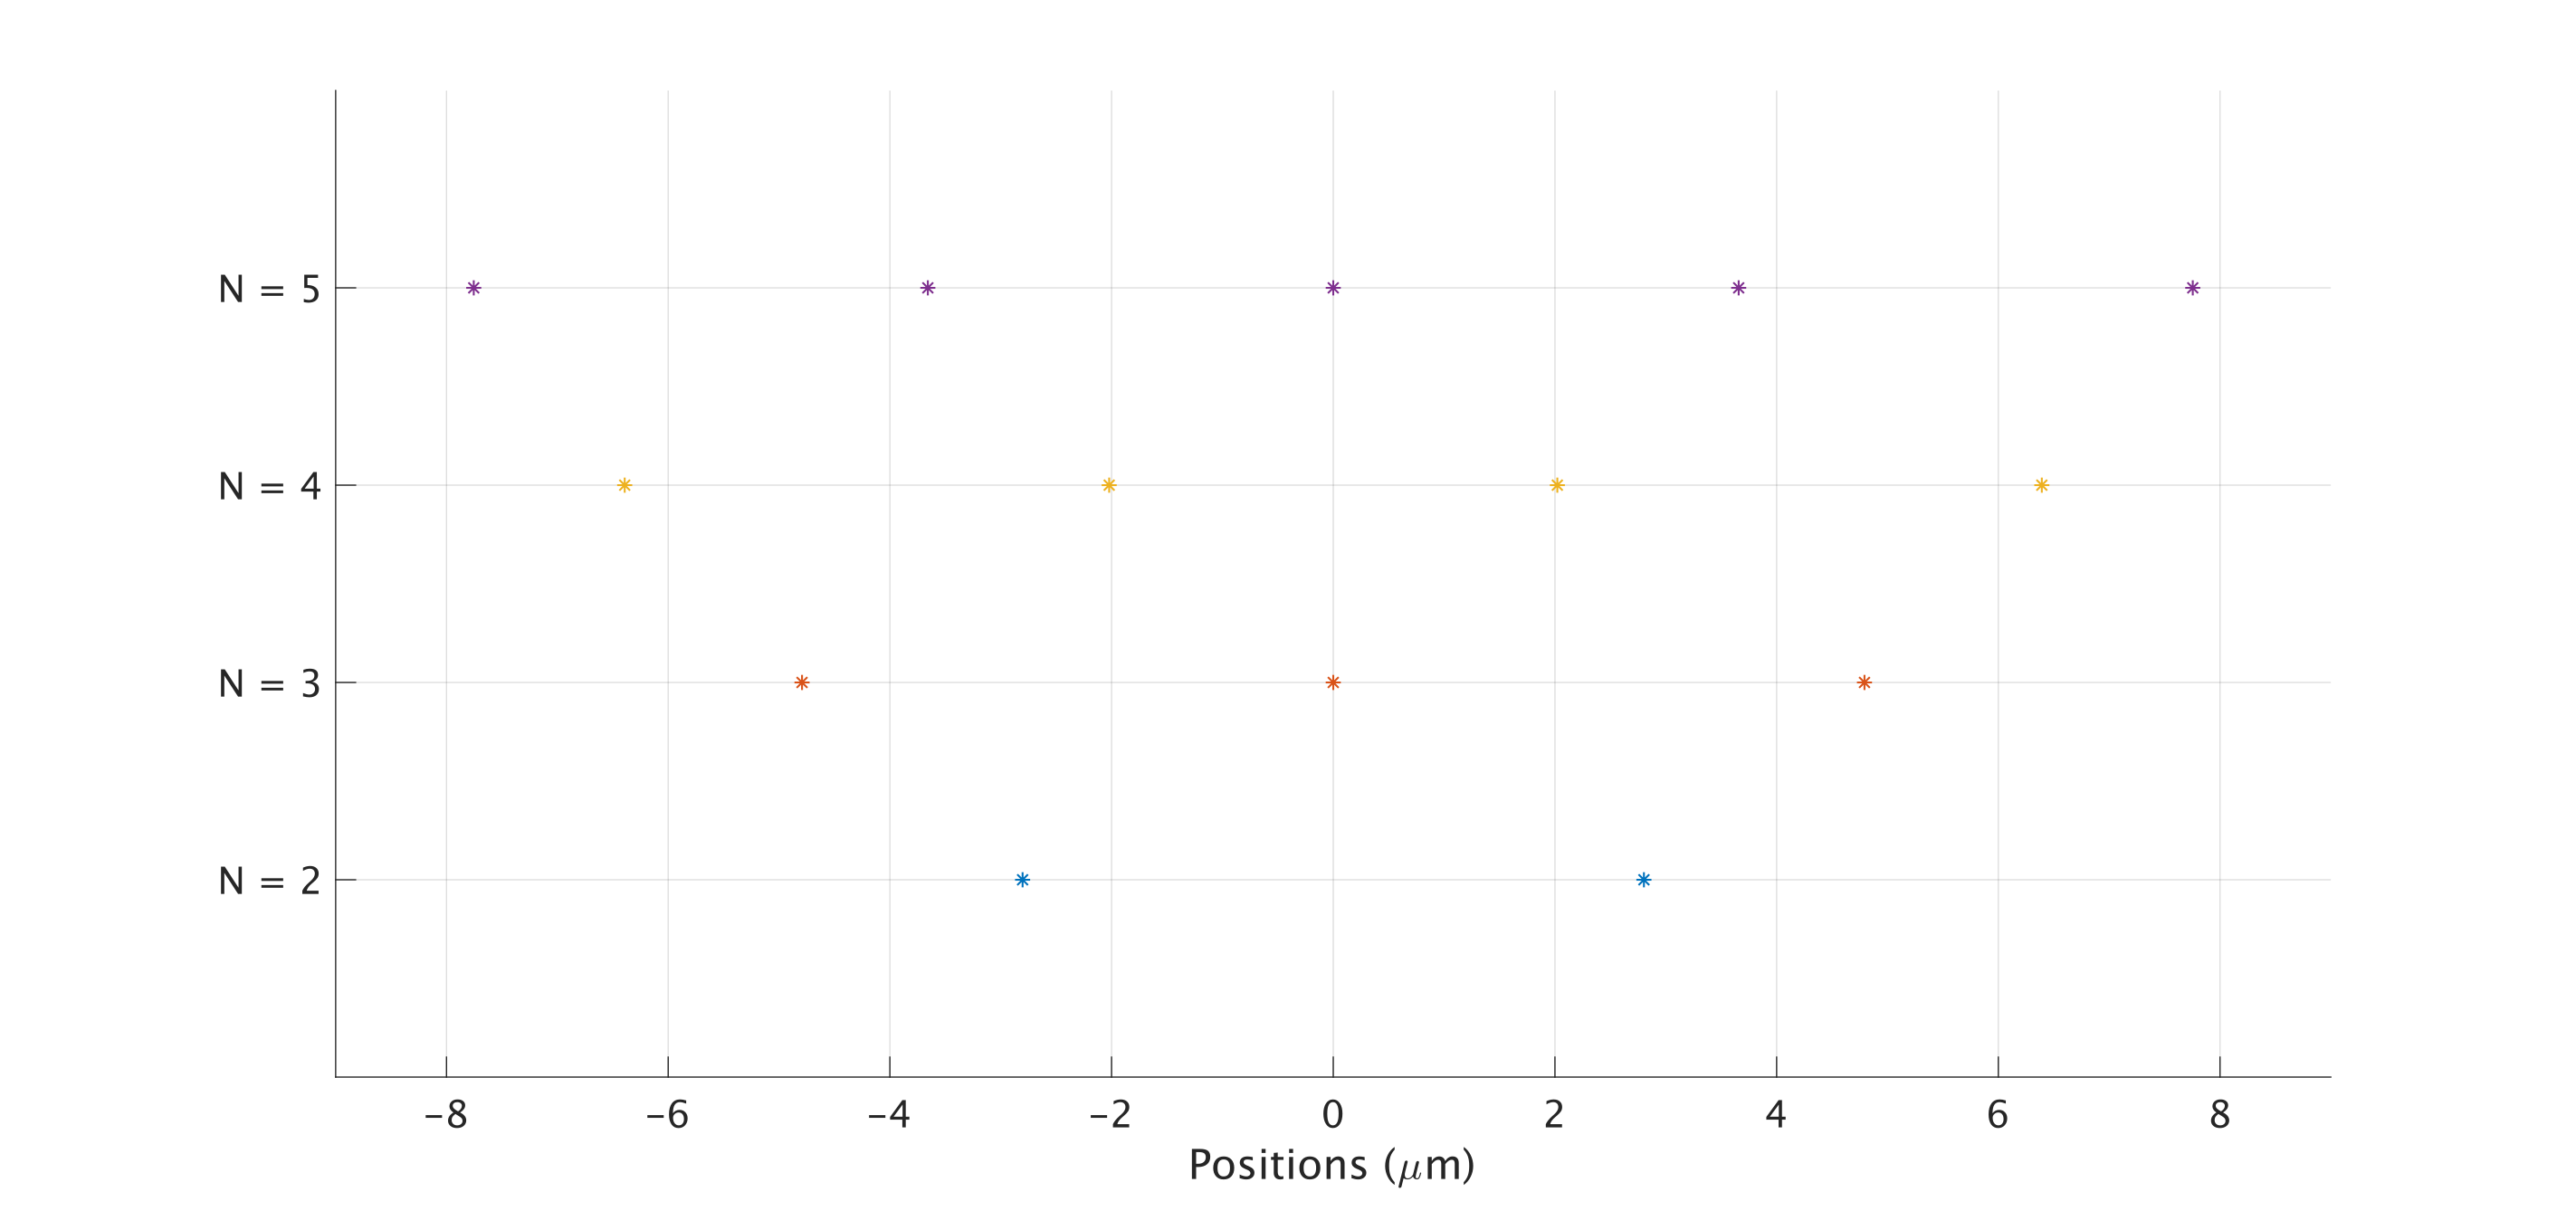
\includegraphics[width = 1.2\textwidth]{positions_ions}
\caption{Ions position for different number $N$ of ions in the trap. Confinement is $\omega_z = 2\pi\times 1$ MHz.}
\label{positions_ions}
\end{figure}


\subsection{Doppler cooling}
\label{sec:doppler_cooling}
Coherent manipulation of ions require cooling them to reach at least the Lamb Dicke regime \cite{Wineland1998}, where the extend of the ion wave packets is much small than the optical wavelengths of the lasers. Several techniques are available for cooling, but the most popular and more frequently used is Doppler cooling. The idea comes from neutral atoms \cite{1975OptCo..13...68H} and can be applied to ions as well: a laser interacts with a particular transition, exchanging a photon and therefore giving a momentum kick $\Delta p = \hbar \mathbf{k}$ in a particular direction to the ion. The absorbed photon is given back through spontaneous emission in a random direction, giving another kick to the ion. Over many cycles of absorption and emission, the random kick due to emission will average to zero, while the kick given by the laser will accumulate slowing down and cooling the ion in the direction of the laser. \\
For describing the Doppler cooling we assume that the ion is weakly confined $\omega \ll \Omega$.\\
The master equation \eqref{masterequation} can be explicitly written for every component of the density matrix $\rho$, in the rotating frame they are called optical Bloch equations and they are
\begin{equation}
\label{rhoee}
\frac{d\rho_{ee}}{dt} = -i\frac{\Omega}{2}(\rho_{eg} - \rho_{ge}) - \Gamma \rho_{ee}
\end{equation}
\begin{equation}
\frac{d\rho_{gg}}{dt} = i\frac{\Omega}{2}(\rho_{eg} - \rho_{ge}) + \Gamma \rho_{ee}
\end{equation}
\begin{equation}
\frac{d\rho_{ge}}{dt} = -\left(\frac{\Gamma}{2}+i\Delta\right)\rho_{ge} -i\frac{\Omega}{2}(\rho_{ee} - \rho_{gg})
\end{equation}
\begin{equation}
\frac{d\rho_{eg}}{dt} = -\left(\frac{\Gamma}{2}-i\Delta\right)\rho_{eg}+i\frac{\Omega}{2}(\rho_{ee} - \rho_{gg})
\end{equation}
We are interested in the steady state case, i.e. when the system reached he equilibrium. Therefore, we look at $\rho_{ee}(t\to \infty) $, the solution of equation \eqref{rhoee} is
\begin{equation}
\rho_{ee}(t\to \infty) = \frac{\Omega^2/\Gamma^2}{1 + \left(2\frac{\Delta -\mathbf{k}\cdot \mathbf{v}}{\Gamma}\right)^2 + 2\frac{\Omega^2}{\Gamma^2}}
\end{equation}
The force exerted on the ions, due to the radiative pressure, is proportional to this population as
\begin{equation}
F = \hbar k \Gamma \rho_{ee} \simeq F_0 + \frac{dF}{dv}v = \hbar k \Gamma\frac{\Omega^2}{\Gamma^2 +4\Delta^2} + F_0 \frac{8k\Delta}{\Gamma^2 + 4\Delta^2}v
\end{equation}
where we assumed low velocities $v \simeq 0$ and thus linearized the equation. The effect of the constant term in the force is just to displace the ion from its central position. Instead, the linear term acts as a viscous friction that cools the ions with a rate of $\dot{E}_c = \braket{Fv}$.
If on one side spontaneous emission allows for Doppler cooling, it also sets the lower limit. The small fluctuations in the Brownian motion leads to diffusion which heats the ion at a rate of
\begin{equation}
\dot{E}_h = \frac{1}{m}\frac{d}{dt}\braket{p^2} =  \frac{1}{m}(\hbar k)^2 \Gamma \braket{\rho_{ee}(v)}.
\end{equation}
At equilibrium, the heating rate equals the cooling rate giving the lowest temperature achievable
\begin{equation}
\dot{E}_h + \dot{E}_c = 0  \implies k_B T = -\frac{\hbar \Gamma}{4}\left(\frac{\Gamma}{2\Delta} +\frac{2\Delta}{\Gamma}\right).
\end{equation}
From here it is clear that by choosing the appropriated detuning, it is possible to reach the lowest temperature
\begin{equation}
T_{min} = \frac{\hbar \Gamma}{2k_{B}}, \qquad \text{for} \quad \Delta = -\frac{\Gamma}{2}.
\end{equation}
At this temperature, the average phonon number is $\braket{\hat{n}} = \Gamma /2\omega_z$ \cite{Eschner:03}. As an example, calcium ions confined in a trap with $\omega_z = 2\pi\times 1$ MHz, can be cooled using the transition $\ket{\text{S}_{1/2}}\to \ket{\text{P}_{1/2}}$ ($\Gamma = 2\pi\times 20.8$ MHz), the Doppler temperature is $T_{min} \sim 500\,\mu$K, and the corresponding average phonon number is $\braket{\hat{n}} = 10.4$. The wavefunction extend for this phonon number can be found as the standard deviation of the operator $\hat{z}$ for the vibrational state $\ket{n}$, creation and annihilation operator algebra gives
\begin{equation}
\sigma_z = \sqrt{\braket{\hat{z}^2}} = \sqrt{\frac{\hbar}{2m\omega_z}(1+2\braket{\hat{n}})} \simeq 52.5\,\text{nm}.
\end{equation}
An ion cooled with Doppler cooling therefore has a spatial dimension still much smaller than the ion separations.\\
To further decrease $\braket{\hat{n}}$, sideband cooling is used \cite{Eschner:03}, here particular sideband transition are excited to reduce the phonon number of the ions inside the trap. However in the experiments of this thesis, only Doppler cooling has been performed.\\


\begin{figure}
\centering
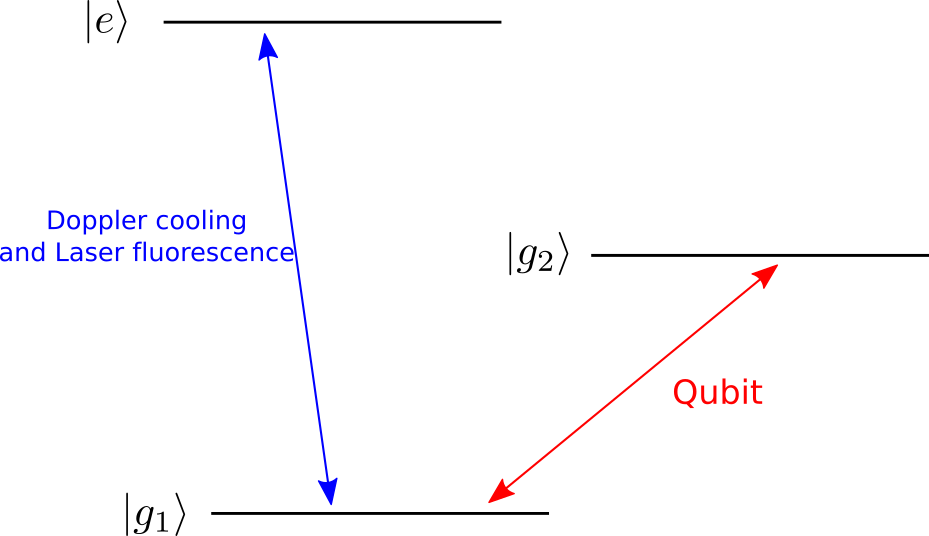
\includegraphics[width = .6\textwidth]{threelevelatom}
\caption{$\Lambda$ type scheme. Two ground states $\ket{g_1}$ and $\ket{g_2}$ are stable or metastable, while the excited level $\ket{1}$ is short lived. Qubit is encoded in the two ground states while laser fluorescence and laser cooling is done on the $\ket{g_1}\to \ket{1}$ transition.}
\label{threelevel}
\end{figure}
\section{Laser beam}
\subsection{Gaussian beams}
\label{sec_diffraction}
Lasers emit light in the shape of Gaussian beams, so it is import to understand what Gaussian beams are and their characteristics. In this chapter we will take a closer look into such beams and introduce important quantities to characterize a Gaussian beam. \\
From a theoretical point of view, Gaussian beams are a particular solution of the Helmholtz equation $(\nabla^2 + k^2)U(\mathbf{r}) = 0$, with $k$ being the wavevector, and $U(\mathbf{r})$ the complex electric field. If we can consider a wave propagating in the $z$ direction, we can write it as \cite{saleh}:
\begin{equation}
\label{gaussianbeams}
U(\mathbf{r}) = A_0 \frac{W_0}{W(z)}\exp\left\{-\frac{x^2+y^2}{W^2(z)}\right\}\exp\left\{-ikz-ik\frac{x^2+y^2}{2R(z)}+i\arctan(z/z_0)\right\}.
\end{equation}
This is the form of Gaussian beams, they are characterized by an amplitude $A_0$, a width $W(z)$, Rayleigh range $z_0$, and a curvature radius $R(z)$. Let us take a look at the features that arise from this shape. The intensity can be calculate by taking the square of the complex amplitude
\begin{equation}
\label{beamintensity}
I(r) = |U(r)|^2 = I_0 \left(\frac{W_0}{W(z)}\right)^2 \exp\left\{\frac{2x^2 + 2y^2}{W^2(z)}\right\}  \qquad I_0 = |A_0|^2.
\end{equation}
It is clear from here why the beam is called Gaussian. For a fixed $z$, i.e. the sections in the $x-y$ plane are shaped as a two dimensional Gaussian distribution.
Therefore, one dimensional Gaussian can be found as cross section of the 2D profile. For simplicity, let us take the profile for a fixed $z$ and $y=0$, this takes the form
\begin{equation}
I(x,y=0,z) = \widetilde{A}(z) \exp\left\{\frac{2x^2}{W^2(z)}\right\} \qquad \widetilde{A}(z) = I_0 \left(\frac{W_0}{W(z)}\right)^2  .
\end{equation}
In figure \ref{gauss}, the $x$ cross section is depicted for this intensity profile normalized in amplitude, and with $\sigma = 1$, $z=0$. Parameters used to measure the width are also displayed and defined in the caption. All of those quantities are equivalent and differ only by a prefactor, so for the rest of the section, we stick to $W(z)$ and study its behaviour.
\begin{figure}
\centering
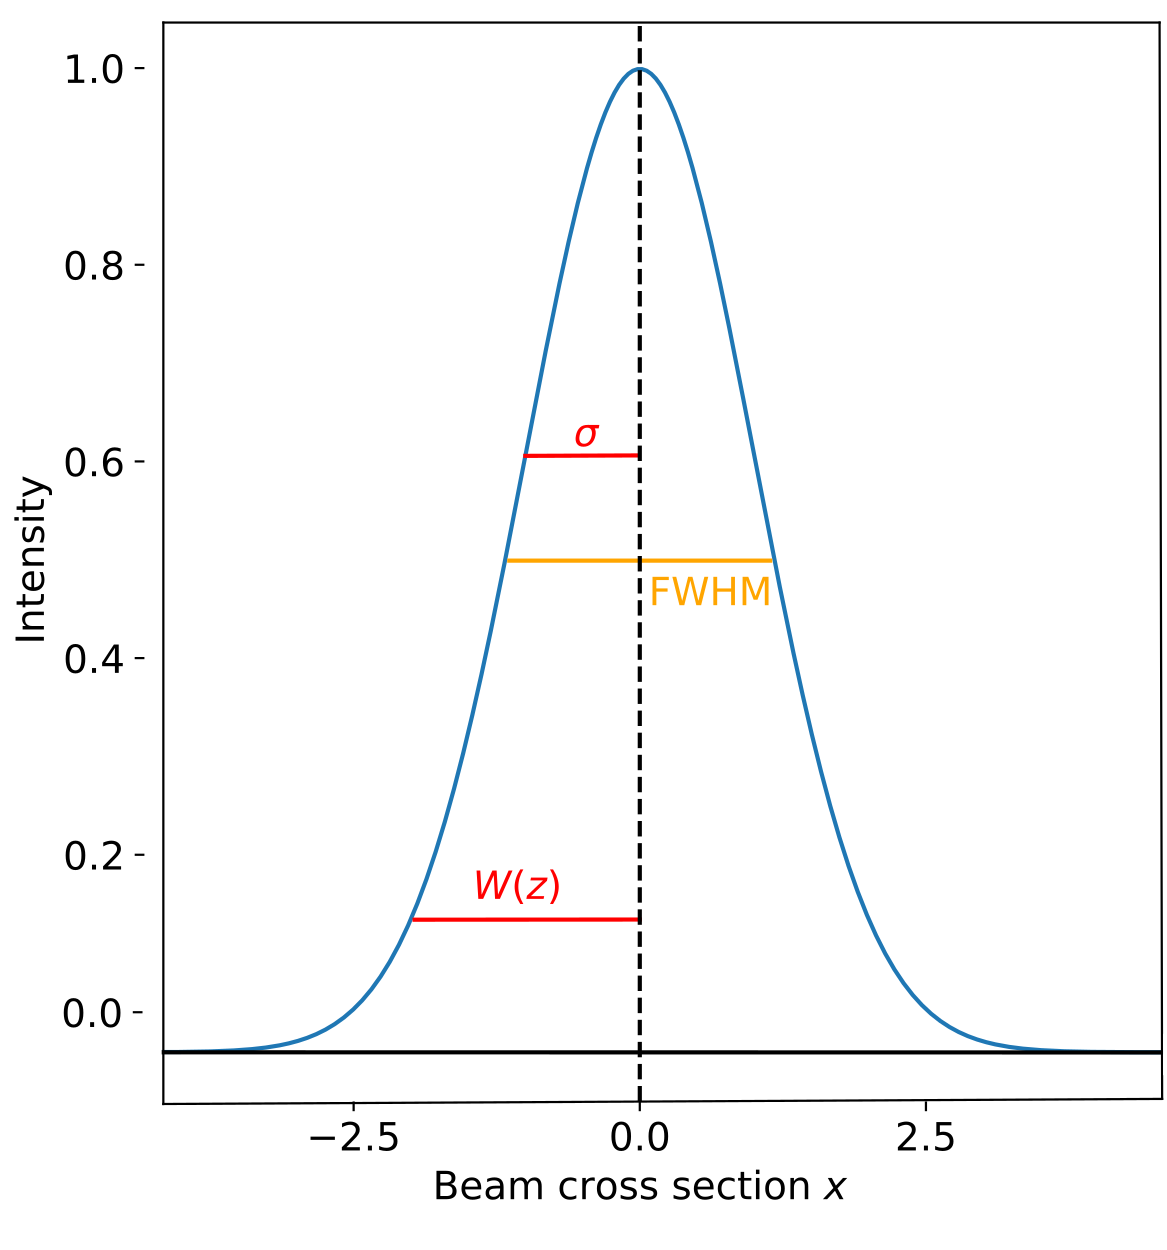
\includegraphics[width = .6\textwidth]{gauss2}
\caption{Intensity of a Gaussian beam, $x$ cross section. The beam is normalized and $\sigma=1$. Graphical representations of used widths are displayed: $W(z)$ is defined as the point at which the intensity $I$ has fallen to $1/e^2 = 13.5\%$ of its maximum value; $\sigma$ is the standard deviation of a Gaussian in the form $Ae^{-\frac{x^2}{2\sigma^2}}$; FWHM is the full width half maximum. Relationships among these quantities are: $W(z) = 2\sigma$, and $W = 0.84\cdot \text{FWHM}$.}
\label{gauss}
\end{figure}
From Helmholtz equation \cite{saleh}, the profile of $W(z)$ as a function of $z$ is found to be
\begin{equation}
\label{waistprofile}
W(z) = W_0 \sqrt{1 + \left(\frac{z}{z_0}\right)^2}\qquad W_0 = \sqrt{\frac{\lambda z_0}{\pi}} \qquad z_0 = \frac{\pi W_0^2}{\lambda}.
\end{equation}
$\lambda$ is the wavelength, and $W_0$ and $z_0$ are respectively the waist of the beam and the Rayleigh range discussed below.\\
There are important features to be noticed with reference to figure \eqref{gaussprofile}:
The width $W(z)$ assumes its minimum value $W_0$ at $z=0$, this spot is called focus and its width $W_0$ is the waist of the beam. The Rayleigh range $z_0$ gives an idea of how quickly the beam is expanding. Mathematically $z_0$ is the distance between the focus and the point where the width $W(z)$ is exactly $\sqrt{2}W_0$.
For $z \gg z_0$, the beam profile diverges almost linearly with an angle given by $\theta = W_0/z_0$, which means the smaller the focus, the greater it diverges.\\
This property will become important later in the work, because it provides one limit on the focus spot. In fact, the optical aperture of the trap is limited by the electrodes, and a beam that diverges too rapidly can potentially clip on one electrode causing aberrations and scattered light in the whole trap.\\
A Gaussian beam can be shaped using optical elements.
\begin{figure}
\centering
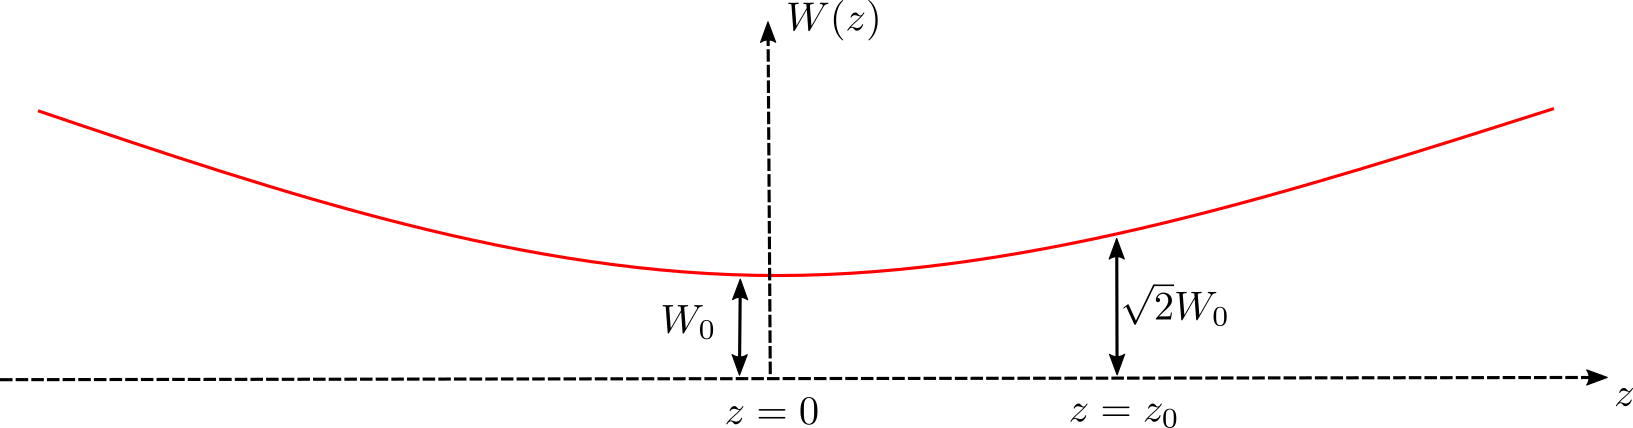
\includegraphics[width = \textwidth]{gaussprofile}
\caption{Width profile of a Gaussian beam, equation \eqref{waistprofile}. The beam is focused at the position $z_0$, here it assumes the minimum width $W_0$, also referred to as waist.}
\label{gaussprofile}
\end{figure}
In order to study such reshaping, let us consider a thin spherical lens with focal length $f$, and radius of curvature $R_l$ placed at position $z$. The effect of the lens on the beam is to give an extra phase factor $k(x^2 + y^2)/2f$ to equation \eqref{gaussianbeams} \cite{beamparameters}. We can match the phase of the incoming and emerging waves, which have respectively radius of curvature $R$, and $R'$, this results in
\begin{equation}
\frac{1}{R'} = \frac{1}{R} - \frac{1}{f}.
\end{equation}
The effect of the lens is to change the radius of curvature to $R'$. Moreover, the width of the beam at the lens is not altered $W=W'$. Using these last two facts, we can determine all the parameters of the outgoing wave. The most important for us is the new waist $W_0'$
\begin{equation}
W_0' = MW_0 \qquad M = \frac{M_r}{\sqrt{q+r^2}} \qquad M_r = \left|\frac{f}{z-f}\right| \qquad r = \frac{z_0}{z-f}.
\end{equation}
$M$ is the magnification factor which provides an easy way to describe the change of the beam. For a better understanding of this last result, let us consider an less general example. We place the lens at the focus $z=0$, and have a collimated beam $z_0 \to +\infty $. In this case the new waist is
\begin{equation}
\label{eq:newwaist}
W_0' = \frac{W_0}{\sqrt{1 + (z_0/f)^2}} \simeq W_0\frac{f}{z_0} = \frac{\lambda f}{\pi W_0}
\end{equation}
where the approximation comes from taking $z_0\gg f$. There are three parameters we can act on to achieve the smallest focus spot: (a) the wavelength $\lambda$, the shorter the better; (b) the focal length of the lens $f$, smaller focus with shorter focal length; (c) the waist of the incoming beam $W_0$, larger waist corresponds to narrower focus.\\
An optical system performing to the theoretical limit is said to be diffraction limited. In the instance of a focusing system, it corresponds to the case where the collimated beam diameter $2W_0$ is equal to the diameter $D$ of the focusing lens. Equation \ref{eq:newwaist} becomes
\begin{equation}
W_0 = \frac{2\lambda}{\pi} \frac{f}{D}.
\end{equation}
If the size of the collimated beam is further increased, the lens becomes a finite size aperture and diffraction effects will appear at the image plane.
%An a numerical example, the objective used in this thesis setup has an aperture of 40 mm, focal length of 54 mm, therefore for a wavelength of $\lambda = 393$ nm the best achievable waist is $1.02\,\mu$m.

\subsection{Beam stearing via Acousto-optical Deflectors}
\label{theory_AOD}
An acousto-optical deflector (AOD) is a common device that can change the propagation direction of a laser beam, typically on the few microsecond timescale. In this work we use an AOD to change which ion is illuminated by a single-ion focused laser. The working principle of an AOD is based on the Acousto-optical effect. A piezo is used to create acoustic waves that propagate through a crystal. The waves modify the crystal refractive index, creating a periodic optical grating that can deflect light travelling through it.  \\
Following the approach of \cite{saleh} to model the device, let us consider a rectangular crystal like in figure \ref{AOD}. The acoustic wave creates a sinusoidal pattern with frequency $\Omega_s$ and wavevector $q$, for the refractive index $n(x,t)$
\begin{equation}
n(x,t) = n - \Delta n_0 \cos \left(\Omega_s t - qx \right),
\end{equation}
where $n$ is the refractive index of the unperturbed medium, $\Delta n_0$ is the amplitude of the perturbation. $\Delta n_0$ is proportional to the square root of the sound intensity.
\begin{figure}[H]
\centering
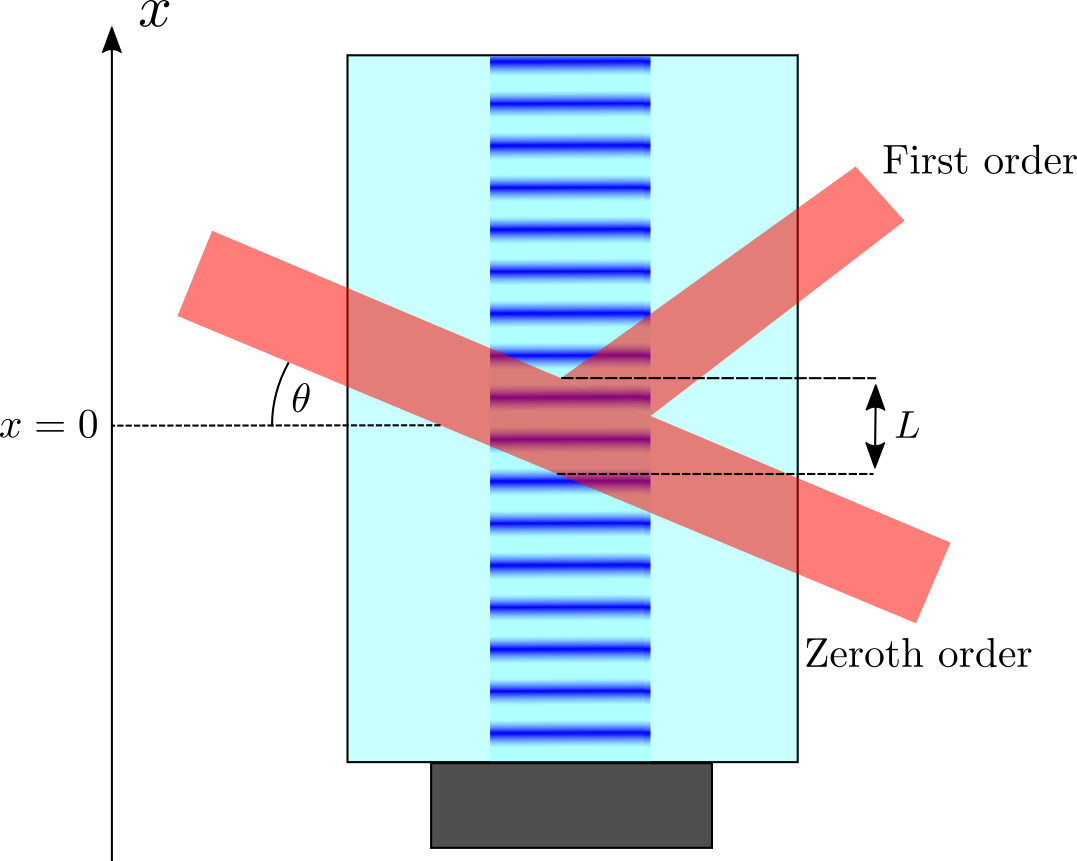
\includegraphics[width = .5\textwidth]{aod2}
\caption{Simple model of an AOD. In black at the bottom a black piezo that generates acoustic waves through the light blue crystal. In red, a collimated beam of light enters in the crystal with an angle $\theta$ and gets partially deflected due to the interaction with the effective optical grating created by the acoustic waves.}
\label{AOD}
\end{figure}
The complex amplitude of the refracted wave $r$ can be calculated by dividing the crystal in thin layers, each with his refractive index $n(x)$. The total refraction is given by all the contributions $\frac{dr}{dx}$ of every layer, we can therefore integrate in the $x$ direction over the length $L$ as follow:
\begin{equation}
r = \int_{L/2}^{L/2} e^{i2kx \sin\theta} \frac{dr}{dx} \,dx
\end{equation}
The included phase takes into consideration the different phase of the input beam when different layers are met. The integral can be solved with a change of variable
\begin{equation}
\frac{dr}{dx} = \frac{dr}{dn}\frac{dn}{dx} = \frac{dr}{dn} q \Delta n_0 \sin \left(\Omega_s t - qx \right),
\end{equation}
The sine function can be written as exponential and now the integral contains only exponential functions which are trivial to calculate. At the end we obtain two contributions for the refracted wave $r$:
\begin{equation}
\label{mainAOD}
r = r_+ + r_- \qquad r_\pm = \pm i r_0 \text{sinc} \left[(2k\sin\theta \mp q)\frac{L}{2\pi} \right]e^{\pm i\Omega_s t}
\end{equation}
These two terms are the plus and minus first order diffraction, an acousto-optical device can be operated symmetrically entering either with a positive angle or with a negative one. Since the maths and the physics is the same, we will focus only on the positive term, called upshifted Bragg diffraction. The sinc function peaks sharply when its argument is 0, i.e. at $2k\sin\theta = q$, and then quickly decreases as the angle is changed. Hence, the input beam must enter with a particular angle in order to diffract with maximum efficiency. The condition to be satisfied is usually called Bragg condition, and can be written as a function of the optical $\lambda$ and acoustic $\Lambda_s$ wavelengths as
\begin{equation}
\label{braggcondition}
\sin \theta  = \frac{\lambda}{2 \Lambda_s} \qquad \Lambda_s = \frac{2\pi}{q}.
\end{equation}
If the condition is not perfectly matched, some light will not be diffracted and will be transmitted unaltered through the device.
The ratio of the transmitted and diffracted light is called diffraction efficiency and gives an idea of how well an acousto-optical device is performing.\\
From equation \eqref{mainAOD} we can notice that an extra phase factor proportional to $\Omega_s t$ is added to the reflected wave. Thus, if the incoming wave is oscillating at $\propto e^{i\omega t}$, the diffracted wave will oscillate as $\propto r_{+}e^{i\omega t} \implies \propto e^{i(\omega + \Omega_s )t}$. The frequency of the diffracted wave $\omega_r$ is therefore shifted by the frequency of the acoustic vibration as
\begin{equation}
\label{eq:aodshift}
\omega_r  =  \omega + \Omega_s.
\end{equation}
The acousto-optical effect described above is common to different devices optimized for specific tasks. Two of the most commons devices are Acousto-optical Deflectors (AOD) and Acousto-optical Modulators (AOM). The idea of the latter is to shift the frequency of a laser using equation \eqref{eq:aodshift}. Deflectors instead exploit the fact that the deflection angle $\theta$ changes linearly as a function of the acoustic frequency $\Omega_s$. Assuming that the angle $\theta$ is small enough to approximate $\sin\theta \sim \theta$, the Bragg condition can be written as
\begin{equation}
\theta \simeq \frac{\lambda}{2 v_s}f,
\end{equation}
where $v_s$ is the speed of sound and $f$ the frequency of the acoustic wave. We can already see that if we change the frequency $f$, the deflection angle $\theta$ changes proportionally. Although the Bragg condition \eqref{braggcondition} is not satisfied anymore, we can work with small enough angles that the diffraction efficiency remain above a certain thresholds. The bandwidth $B$ specifies the range of frequencies over which deflectors work.\\
AOMs and AODs differ by the relative divergence of the optical and acoustic beam \cite{handbookoptics}, moreover for AODs, speed and the number of resolvable spots are more important, while for AOM's the optimization focus is on modulation bandwidth. These different priorities in building the devices influence
the choice of the crystal and acoustic mode, for instance, a slow acoustic velocity and shear mode are preferred in AODs \cite{handbookoptics}. More advanced techniques to engineer an AOD are available, for example the piezo is replaced by a phase array of transducers that tilt the acoustic beam \cite{phasedarray}.\\
As already stated, in the experiment setup of this work, an AOD is used to steer a single-ion focused laser and aim at different ions in the $\mu$s scale. AOMs instead are extensively used to tune and scan the laser frequency.

\section{Experiments model}
The aim of this thesis is to perform two experiments with ions: qubit manipulation, and photon generation. In addition to test these two functionalities, the experiments are also designed to asses the performance of the addressing system as is discussed below. In both cases a string of 3-4 ions is loaded in the trap, the addressed Raman laser is focused on a single ion and experiments are carried out.

\subsection{Addressed qubit manipulation}
A we have seen, ions can be used to encode and process quantum information. As highlighted in figure (), the qubit is encoded in the $\ket{S} \to \ket{D}$ transition. The 393nm transition from $\ket{S}\to \ket{P}$ can be used to induce a phase shift on the ground state of the qubit $\ket{S}$. In the off resonant regime, the laser induces a Stark shift $\delta = \Omega^2/4\Delta$ without actually exciting the state. As discussed in section \ref{sec:dissipation}, in order for this to happen, we should have $\delta \gg \Gamma_{eff}$. Therefore in the experiment we decided to set the detuning such that the ratio between the Stark shift and the spontaneous scattering rate is 100
\begin{equation}
\frac{\delta}{\Gamma_{eff}} = \frac{2\Delta}{\Gamma} \sim 100 \implies \Delta \sim 3\,\text{GHz}.
\end{equation}
Furthermore, ions can be used as sensitive tools for beam profiling, the addressed manipulation changes only the qubit state of a single ion. Hence, by measuring the state of all ions, and scanning the beam across the ions string, a beam profile can be obtained. In a single experiment we can therefore characterize the beam and demonstrate qubit manipulation.
The experiments consist of Ramsey interferometry, already performed in the past to measure Ac Stark shift \cite{starkshift}.
The idea is to send a resonant $\pi/2$ pulse at 729nm, which bring the qubit state to a superposition $\ket{S}+\ket{D}$, here another in phase resonant $\pi/2$ pulse at 729nm would bring the final state to the excited level $\ket{D}$. However, if between the two 729nm pulses, AC stark shift is induced by a pulse of 393nm light, an additional phase is added to the superposition $\ket{S}+\ket{D}$, and the final state after the second 729nm pulse will depend on the shift induced by the 393nm laser. By calculating the final probability $P_D$ it is possible to infer the power of the 393nm light. Rigorous mathematic can be done with matrices \eqref{laserpulse} here called $U_{729}$ and \eqref{acstarkrotation}, referred to as $U_{393}$. After the three pulse sequence the final state is
\begin{equation}
\begin{split}
\ket{\psi_f} &= U_{729}(\pi,\phi)U_{393}(\delta)U_{729}(\pi,0)\ket{S} \\
&= \frac{1}{2}\left(e^{-i\frac{\delta}{2}t}-e^{-i\phi}\right)\ket{S}-\frac{i}{2}\left(1 + e^{-i\frac{\delta}{2}t} e^{-i\phi}\right)\ket{D}
\end{split}
\end{equation}
where $\delta = \Omega^2/4\Delta$ is the Stark shift, and $\Omega$ is the Rabi frequency of the 393nm light that we want to measure. The final probability is then
\begin{equation}
P_D = \cos^2\left(2\phi + 2\frac{\delta t}{2}\right) = \cos^2\left(2\phi + \frac{\Omega^2 t}{4\Delta}\right).
\end{equation}
As we can see, the final signal depends on the phase of the second 729nm pulse $\phi$ and on the Stark shift induced by the 393nm laser. To get $\Omega^2$ a simple formula inversion can be done
\begin{equation}
\label{eq:ptointensity}
\Omega^2 = \left[\text{arccos}\left(\sqrt{P_D}\right)-2\phi \right].
\end{equation}
 The phase $\phi$ can be set experimentally and all constants have been dropped as the data will be normalized.\\
\begin{figure}
\centering
\includegraphics[width=\textwidth]{sequence}
\caption{Experiment sequence}
\label{sequence}
\end{figure}
The experiment sequence is in figure \ref{sequence}, for every sequence, a stage of Doppler Cooling at the beginning is included, and at the end of the pulses state readout with single-ion resolving camera is performed. The sequence is then repeated $N$ times to estimate the excitation probability for every data point. Between the Raman pulse and the second $\pi/2$ pulse, there is also a dead time which can be adjusted to improve signal to noise ratio.\\

\subsection{Addressed photon generation}
The second experiment consists of generating photons from one single ion, using the Raman process described in section \ref{sec:ramanprocess}. In this case the 393nm laser pulse has to be send at the correct frequency to excite the Raman resonance. Detuning of the cavity and laser pulse must be equal as discussed in section \ref{sec:threelevel}. In order to adiabatically eliminate the $P$ state, we set $\Delta \sim 400$ MHz. The Raman resonance is precisely measure with a double pass AOM, and the frequency is set accordingly. Note that the effective Rabi frequency is proportional to the laser drive Rabi frequency $\propto \Omega$ as seen in equation \eqref{omegaeff}. On the contrary, Ac stark shift depends on the Intensity $\propto \Omega^2$. Therefore, the addressing error in the two experiments are different. After the excitation and photo emission, state detection on all ions is performed, this give the possibility the check if other ions have been unwantedly addressed.
